\begin{figure*}[h]
    \center{
    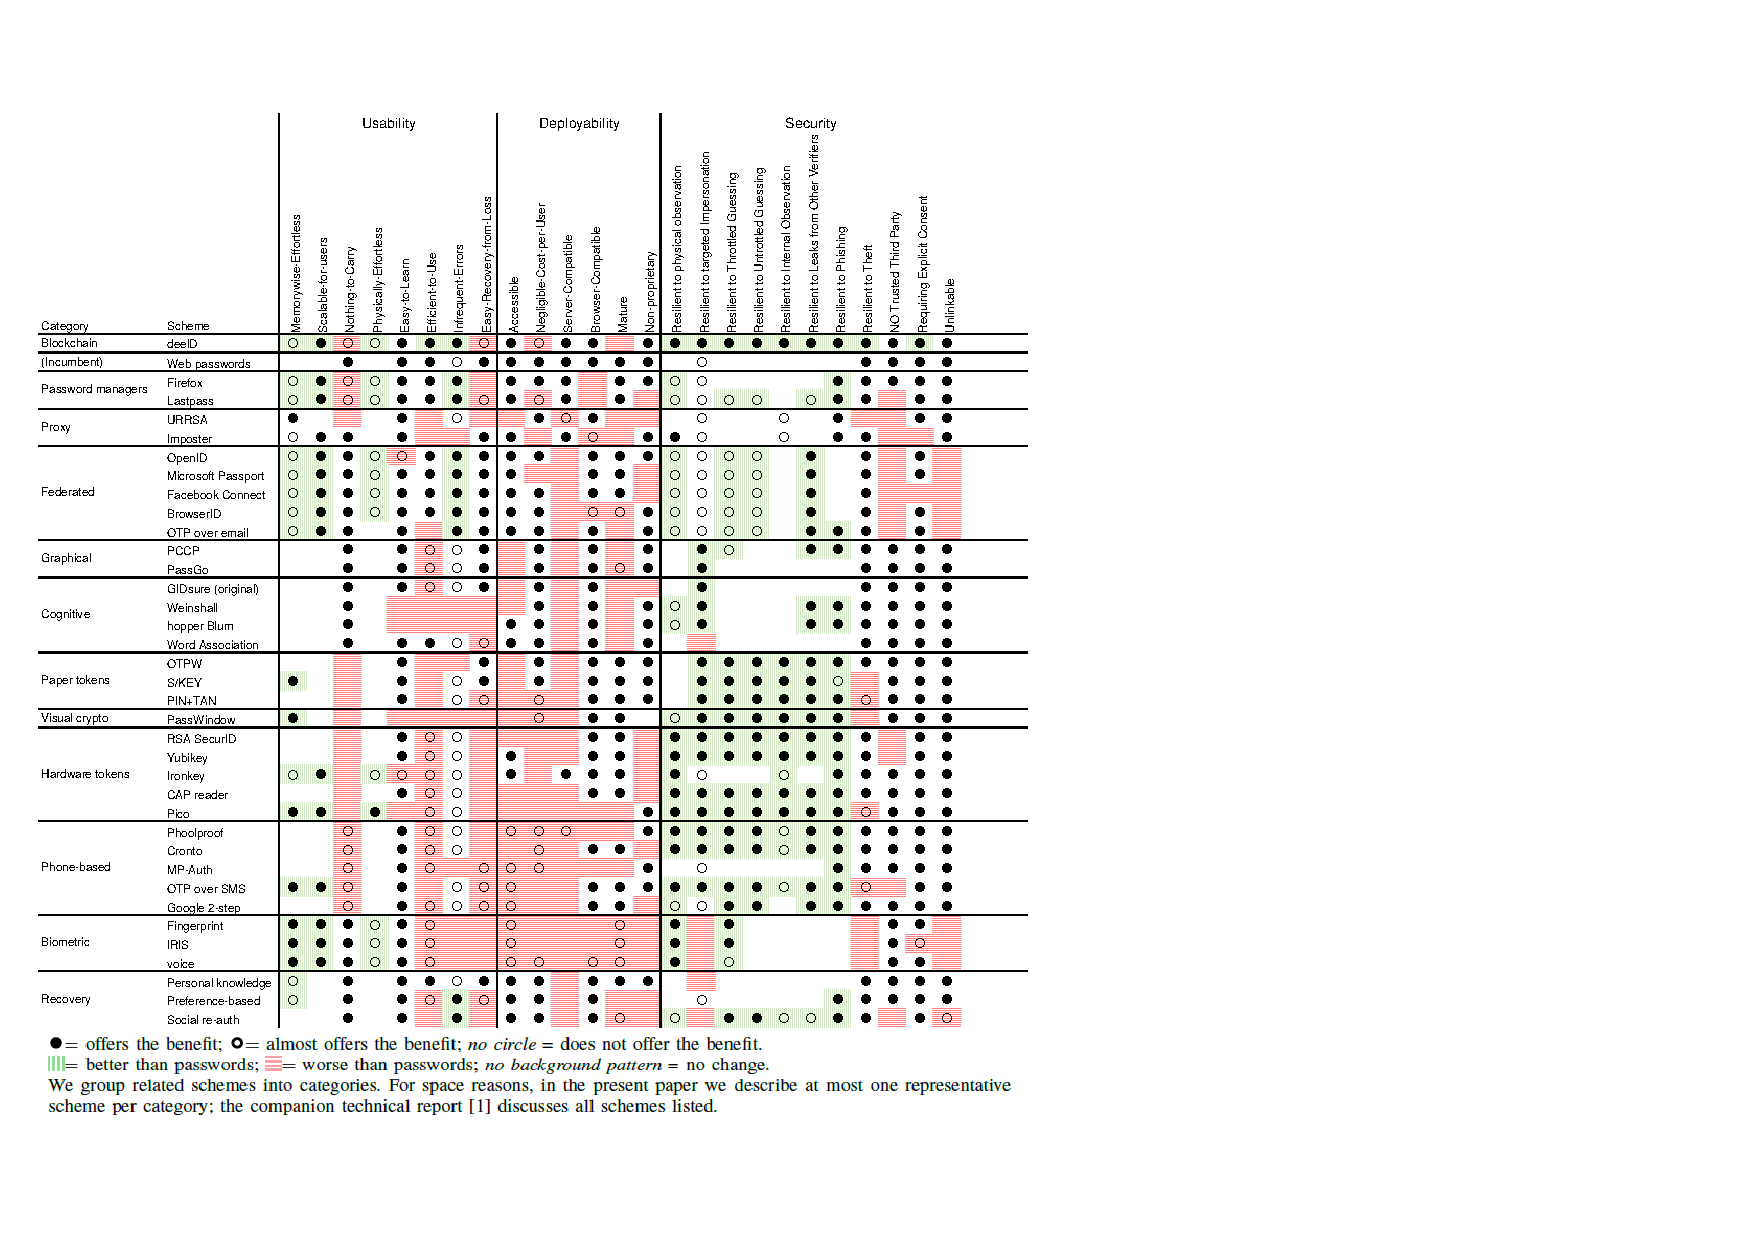
\includegraphics[trim={0 2cm 12cm 1cm},clip, scale=1]{figs/deeid/deeIDComparisonTable3.pdf}}
    \caption{Visual evaluation of various schemes and our new blockchain-based scheme (\deeid).}
    \label{fig:deeIDComp}
\end{figure*}

In \textit{The Quest to Replace Passwords}~\cite{bonneau_quest_2012}, Bonneau~\etal introduce a comprehensive framework to evaluate a wide range of authentication schemes, with particular emphasis on those employed in web-based environments. In the following section, we extend this analysis rigorously applying the framework to \deeid, critically examining its security properties, usability considerations, and overall performance in the context of modern authentication challenges.

Starting with \textit{Usability benefits}, we believe \deeid provides \textit{Memorywise-Effortless} benefits, as there is no need to remember a password or secret. However, for enhanced security, we encourage users to maintain a PIN-protected device. The application is highly scalable for users, who can store unlimited credentials without additional burden, making it superior to passwords. Whilst users are required to carry a device, such as a mobile phone, this is an object they typically carry. The scheme is also \textit{Physically-Effortless}, as users need only aim their device and press a button to grant or decline a request. The scheme is also \textit{Easy-to-Learn} and intuitive, requiring only image scanning and pressing of the button. Moreover, it is much more efficient than passwords, \textit{Efficient-to-Use}, as users need only scan and press a button, rather than type or recall a password. Regarding \textit{Infrequent-Errors}, particularly compared to biometric schemes, the process is highly reliable with no false positives. However, the scheme presents challenges regarding the recovery of lost private keys; depending on which keys are lost, recovery methods are typically unavailable, necessitating replacement of lost credentials with the identity provider.

Moving onto \textit{Deployability benefits}: The scheme is highly \textit{Accessible} and provides \textit{Negligible-Cost-per-User}; beyond access to a mobile phone device, users incur no additional expenses, which applies equally to the verifier. The scheme is also \textit{Server-Compatible}, meaning organisations can implement it using their existing technology. At the prover's end, no browser modifications are required, therefore it is \textit{Browser-Compatible}. Although it is not proprietary technology, it has not yet reached maturity at this stage.

On \textit{Security-benefits}: The scheme is resilient to physical observations, as the secret is unobservable and all authentications occur without revealing secret keys. It demonstrates resilience to targeted impersonation, as knowledge of personal details cannot compromise the authentication scheme. Given that the scheme is challenge-response based and operates machine-to-machine (mobile phone to server), the failure rate for reasons other than incorrect keys is minimal, thus making successful guessing highly improbable. Unthrottled-guessing vulnerability depends on the identity provider and their key lengths. Resilient-to-Internal-Observation is notably robust, as users do not interact directly with private keys, rendering key logging and similar methods ineffective at revealing the secret key. Following the zero-knowledge principle of the Fiat--Shamir concept, information known to the verifier cannot reveal any details about the user's secret key. The scheme demonstrates resilience to phishing attacks, again due to zero-knowledge properties, as no secret-key information is revealed. Although the scheme shows less resilience to theft, the implementation of PIN protection renders it quasi-resilient-to-theft. Regarding \textit{No-Trusted-Third-Party}: the scheme operates independently of trusted third parties beyond the initial identity provision, eliminating their control and influence thereafter; should they become compromised, it merely necessitates discontinuing acceptance of identities from the newly untrusted third party. The scheme requires explicit user consent for authentication (requiring physical button activation after device log-in). In the absence of an authenticator, services cannot determine whether the same user is accessing various platforms. However, should verifiers collaborate and share user information, they could identify common users across their services. Crucially, the authentication scheme itself does not facilitate user linking.